%------------------------------------------------------------
\title[03 - 进制]
{03 - 进制}

\subtitle{C++ 程序设计进阶}

\author[Beiyu Li]
{Beiyu Li\\
\texttt{<sysulby@gmail.com>}}

% \institute[SOJ]
% {Sicily Online Judge}

\date[\today]
{\number\year 年 \number\month 月 \number\day 日}
%------------------------------------------------------------


\begin{document}

\author[sysulby]
{SOJ 信息学竞赛教练组}

\begin{frame}
    \titlepage
\end{frame}
\setcounter{framenumber}{0} % 标题页不编号

\section{复习回顾}

%------------------------------------------------------------
\begin{frame}[fragile]
    \frametitle{变量}

    \begin{itemize}
        \item<1-> 作用域
            \begin{itemize}
                \item 局部变量:从变量的声明开始到包含它的块结束
                \item 全部变量:从变量的声明开始一直到代码结束
            \end{itemize}

        \item<2-> 同名变量
            \begin{itemize}
                \item<2-> 一般在什么情况下使用同名变量?
                \item<3-> 变量的作用域完全不重叠
            \end{itemize}

        \item<4-> 引用变量
            \begin{itemize}
                \item 引用变量是其他变量的别名,与其他变量共用同一块内存空间
                \item 修改引用变量的值也会同时修改它所绑定的一般变量的值
                \item 一般用于函数参数传递
            \end{itemize}
    \end{itemize}

\end{frame}
%------------------------------------------------------------

%------------------------------------------------------------
\begin{frame}[fragile]
    \frametitle{函数参数传递}

    \begin{columns}
    
        \column{.7\textwidth}
        \begin{itemize}
            \item<1-> 按值传递
                \begin{itemize}
                    \item 函数中不能修改实参的值
                \end{itemize}
    
            \item<2-> 按引用传递
                \begin{itemize}
                    \item 函数中可以修改实参的值
                    \item 形参变量名前加 \lstinline|&|,实参不用加
                \end{itemize}
    
            \item<3-> 数组传递
                \begin{itemize}
                    \item 本质是传递数组首地址,函数中可以修改实参数组
                    \item 形参数组名后加 \lstinline|[]|,实参不用加
                \end{itemize}
        \end{itemize}

        
        \column{.3\textwidth}
        \only<1>{\lstinputlisting[basicstyle=\ttfamily\scriptsize,language=C++,name=para]{ch15/para.cc}}
        \only<2>{\lstinputlisting[basicstyle=\ttfamily\scriptsize,language=C++,name=refer_para]{ch15/refer_para.cc}}
        \only<3>{\lstinputlisting[basicstyle=\ttfamily\scriptsize,language=C++,name=array_para]{ch15/array_para.cc}}
        \begin{tikzpicture}[remember picture,overlay]
                \only<1>{\redbox{para}{3}{8}{3}{12};}
                \only<1>{\redbox{para}{9}{5}{9}{5};}
                \only<2>{\redbox{refer_para}{3}{8}{3}{13};}
                \only<2>{\redbox{refer_para}{9}{5}{9}{5};}
                \only<3>{\redbox{array_para}{3}{8}{3}{14};}
                \only<3>{\redbox{array_para}{10}{5}{10}{5};}
       \end{tikzpicture}
    
    \end{columns}

\end{frame}
%------------------------------------------------------------

\section{进制的概念}

%------------------------------------------------------------
\begin{frame}[fragile]
    \frametitle{讨论}

    \begin{block}{}
        \vspace{.5cm}
        \begin{center}
            {\Large 为什么日常见到的数字都由 $0 \sim 9$ 组成?}
        \end{center}
        \vspace{.5cm}
    \end{block}
\end{frame}
%------------------------------------------------------------

%------------------------------------------------------------
\begin{frame}[fragile]
    \frametitle{进制}

    \begin{itemize}[<+->]
        \item 日常生活中数字由 $0 \sim 9$ 组成,$9$ 的下一个数是 $10$,这种 “逢十进一” 的计数方法称为十进制。
        \item 进制是人为定义的带进位的计数方法
        \item $X$ 进制
        \begin{itemize}
           \item 规则:逢 $X$ 进一
           \item $X$ 进制中的 $X$ 也称\textbf{基数}
           \item 数值的每位可由 $X$ 个符号(也称\textbf{数码})组成,分别代表 $0 \sim X-1$ 这 $X$ 个数字
        \end{itemize}
    \end{itemize}

\end{frame}
%------------------------------------------------------------

%------------------------------------------------------------
\begin{frame}[fragile]
    \frametitle{常见的进制}

    \begin{itemize}
        \item 在计算机中,常见的有二进制、八进制、十六进制
        \item<2-> 二进制
        \begin{itemize}
           \item 逢二进一,由 $0 \sim 1$ 这 $2$ 个数码组成
        \end{itemize}
        \item<3-> 八进制
        \begin{itemize}
           \item 逢八进一,由 $0 \sim 7$ 这 $8$ 个数码组成
        \end{itemize}
        \item<4-> 十六进制
        \begin{itemize}
           \item 逢十六进一,需要 $16$ 个数码来表示 $0 \sim 15$,通常用 $A \sim F$ 或 $a \sim f$ 表示 $10 \sim 15$
        \end{itemize}
    \end{itemize}

\end{frame}
%------------------------------------------------------------

%------------------------------------------------------------
\begin{frame}[fragile]
    \frametitle{权重}

    \begin{itemize}[<+->]
        \item 以十进制的 $2157$ 为例
        \begin{itemize}
           \item $(2157)_{10} = 2 \times 10^3 + 1 \times 10^2 + 5 \times 10^1 + 7 \times 10^0$
           \item 不同位置上的数字有不同的 “份量”,也称\textbf{权重}
           \item 十进制个位的权重是 $10^0$,十位的权重是 $10^1$,百位的权重是 $10^2$……
        \end{itemize}
        \item 八进制的 $(2157)_8 = ?$
        \begin{itemize}
           \item $(2157)_{8} = 2 \times 8^3 + 1 \times 8^2 + 5 \times 8^1 + 7 \times 8^0$
        \end{itemize}
        \item $(2157)_{10}$ 与 $(2157)_{8}$ 的\textbf{数值}大小不同
    \end{itemize}

\end{frame}
%------------------------------------------------------------

\section{二进制}

%------------------------------------------------------------
\begin{frame}[fragile]
    \frametitle{计算机与二进制}

    \begin{itemize}[<+->]
        \item 计算机底层只使用 $0$ 和 $1$ 两个数字,这样做的原因有:
        \begin{itemize}
           \item 二进制只有两种状态,使用两个稳定状态的物理器件就可以表示二进制的每一位,制作成本比较低,例如用高低电平可以表示 $1$ 和 $0$
           \item 二进制的 $1$ 和 $0$ 正好对应 逻辑的真和假,为计算机实现逻辑运算提供了便利  
        \end{itemize}
        \item 在计算机内部,各种类型的数据(例如整数、实数和字符等)都编码为 $0/1$ 序列 
    \end{itemize}

\end{frame}
%------------------------------------------------------------

%------------------------------------------------------------
\begin{frame}[fragile]
    \frametitle{随堂练习}

    \begin{exampleblock}{选择题}

        \begin{enumerate}
            \item 在计算机内部用来传送、存贮、加工处理的数据或指令都是以什么形式进行的

                \alt<2>{
                    \begin{tasks}
                        \task[A.] \textcolor{red}{二进制码}
                        \task[B.] 八进制码
                        \task[C.] 十进制码
                        \task[D.] 智能拼音码
                    \end{tasks}
                }{
                    \begin{tasks}
                        \task[A.] 二进制码
                        \task[B.] 八进制码
                        \task[C.] 十进制码
                        \task[D.] 智能拼音码
                    \end{tasks}
                }

        \end{enumerate}

    \end{exampleblock}
\end{frame}
%------------------------------------------------------------

%------------------------------------------------------------
\begin{frame}[fragile]
    \frametitle{二进制数的基本运算}

    \begin{itemize}[<+->]
        \item 在加减乘除运算中,二进制数的运算逻辑与十进制数的运算逻辑相同
        \item 区别在于二进制运算是“逢二进一”,十进制运算是“逢十进一”
    \end{itemize}

\end{frame}
%------------------------------------------------------------

%------------------------------------------------------------
\begin{frame}[fragile]
    \frametitle{二进制加法}

    \begin{itemize}
        \item 从低位到高位依次相加,逢二进一
        \begin{itemize}
            \item $0 + 0 = 0$
            \item $0 + 1 = 1$
            \item $1 + 0 = 1$
            \item $1 + 1 = 0$(进位)
        \end{itemize}
        \item<2-> 以 $(10111)_2 + (10001)_2$ 为例

        \uncover<2>{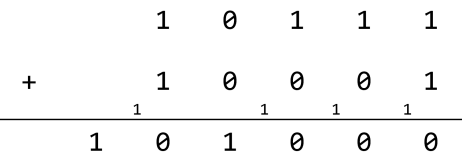
\includegraphics[width=.5\textwidth]{ch15/add.png}}
    \end{itemize}

\end{frame}
%------------------------------------------------------------

%------------------------------------------------------------
\begin{frame}[fragile]
    \frametitle{二进制减法}

    \begin{itemize}
        \item 从低位到高位依次相减,不够则借位,借得 $2$
        \begin{itemize}
            \item $0 - 0 = 0$
            \item $0 - 1 = 1$(借位)
            \item $1 - 0 = 1$
            \item $1 - 1 = 0$
        \end{itemize}
        \item<2-> 以 $(10100)_2 - (1011)_2$ 为例

        \uncover<2>{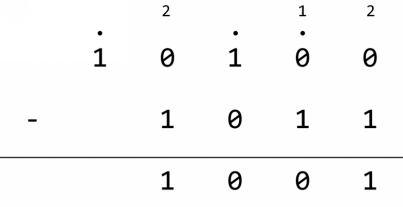
\includegraphics[width=.5\textwidth]{ch15/sub.png}}
    \end{itemize}

\end{frame}
%------------------------------------------------------------

%------------------------------------------------------------
\begin{frame}[fragile]
    \frametitle{二进制乘法}

    \begin{itemize}
        \item 一个乘数的每一位分别乘另一个的每一位,逢二进一
        \begin{itemize}
            \item $0 \times 0 = 0$
            \item $0 \times 1 = 0$
            \item $1 \times 0 = 0$
            \item $1 \times 1 = 1$
        \end{itemize}
        \item<2-> 以 $(101)_2 \times (111)_2$ 为例

        \uncover<2>{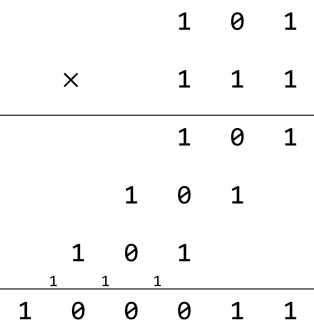
\includegraphics[width=.3\textwidth]{ch15/mul.png}}
    \end{itemize}

\end{frame}
%------------------------------------------------------------

%------------------------------------------------------------
\begin{frame}[fragile]
    \frametitle{二进制除法}

    \begin{itemize}
        \item 从被除数的高位到低位一直除以除数,如果某一位不够除,就包含后一位继续除
        \begin{itemize}
            \item 通过乘法和减法实现
        \end{itemize}
        \item<2-> 以 $(1011)_2 \div (11)_2$ 为例

        \uncover<2>{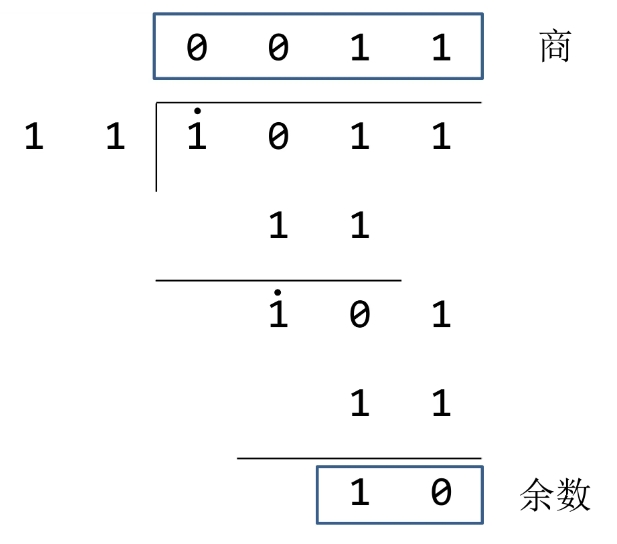
\includegraphics[width=.5\textwidth]{ch15/div.png}}
    \end{itemize}

\end{frame}
%------------------------------------------------------------

%------------------------------------------------------------
\begin{frame}[fragile]
    \frametitle{随堂练习}

    \begin{exampleblock}{选择题}

        \begin{enumerate}
            \item 二进制数 00100100 和 00010101 的和是多少

                \alt<2>{
                    \begin{tasks}
                        \task[A.] 00101000
                        \task[B.] 001010100
                        \task[C.] 01000101
                        \task[D.] \textcolor{red}{00111001}
                    \end{tasks}
                }{
                    \begin{tasks}
                        \task[A.] 00101000
                        \task[B.] 001010100
                        \task[C.] 01000101
                        \task[D.] 00111001
                    \end{tasks}
                }

        \end{enumerate}

    \end{exampleblock}
\end{frame}
%------------------------------------------------------------

\section{二进制整数与十进制整数的转换}

%------------------------------------------------------------
\begin{frame}[fragile]
    \frametitle{二进制转十进制}

    \begin{itemize}
        \item 一个数的数值等于各个数码与其对应的权重乘积之和
        \begin{itemize}
           \item $(2157)_{10} = 2 \times 10^3 + 1 \times 10^2 + 5 \times 10^1 + 7 \times 10^0$
        \end{itemize}
        \item<2-> 二进制每个位的权重是 2 的幂
        \begin{itemize}
           \item $(10011)_{2} = 1 \times 2^4 + 0 \times 2^3 + 0 \times 2^2 + 1 \times 2^1 + 1 \times 2^0$
           \item 计算这个展开式的十进制结果,该结果就是原二进制数对应的十进制数值
           \item $(10011)_{2} = 1 \times 16 + 0 \times 8 + 0 \times 4 + 1 \times 2 + 1 \times 1 = 19$
        \end{itemize}
        \item<3-> 这种二进制转十进制的方法称为\textbf{按权展开求和}
    \end{itemize}

\end{frame}
%------------------------------------------------------------

%------------------------------------------------------------
\begin{frame}[fragile]
    \frametitle{例 3.1:二进制转十进制}

    \alt<2-6>{
        \alt<2-5>{
            \begin{exampleblock}{编程题}
    
                \begin{itemize}
                    \item 思考如何写代码计算以下展开式?
                    \begin{itemize}
                       \item $(10011)_{2} = 1 \times 2^4 + 0 \times 2^3 + 0 \times 2^2 + 1 \times 2^1 + 1 \times 2^0$
                    \end{itemize}
                \end{itemize}

                \centering
                \renewcommand{\arraystretch}{1.2} %设置垂直内边距为1.2倍默认行高
                \begin{tabular}{|c|c|c|c|c|c|}
                \hline
                数位  & 1 & 0 & 0 & 1 & 1 \\ \hline
                权重  & $2^4$ & $2^3$ & $2^2$ & $2^1$ & $2^0$  \\ \hline
                加数 & $1 \times 2^4$ & $0 \times 2^3$ & $0 \times 2^2$ & $1 \times 2^1$ & $1 \times 2^0$  \\ \hline
                \end{tabular}

                \begin{itemize}
                    \item 实现
                    \begin{itemize}
                       \item<3-> 用数组存储二进制的每位,并从低位到高位遍历(倒序遍历)
                       \item<4-> 同时,用变量 $w$ 存储权重,初始化为 $1$($2^0$),且实现每次 $w *= 2$ 的变化
                       \item<5-> 用变量 $sum$ 记录十进制数值,每次把数位与权重的乘积累加到 $sum$ 中
                    \end{itemize}
                \end{itemize}
            \end{exampleblock}
        }{
            \lstinputlisting[basicstyle=\ttfamily\scriptsize,language=C++,name=bin2dec]{ch15/bin2dec.cc}
        }
    }{
        \begin{exampleblock}{编程题}

            \begin{itemize}
                \item 输入一个正整数 $n$ ($1 \le n \le 31$),表示有一个 $n$ 位的二进制数,接下来从高位到低位输入该二进制数的每一位 $a_i$ ($0 \le a_{i} \le 1$)。\\
                    输出该二进制数对应的十进制数值。

                \item 样例输入

                    \lstinline|5|\\
                    \lstinline|1 0 0 1 1|

                \item 样例输出

                    \lstinline|19|

            \end{itemize}

        \end{exampleblock}
    }
\end{frame}
%------------------------------------------------------------

%------------------------------------------------------------
\begin{frame}[fragile]
    \frametitle{十进制转二进制}

    \begin{itemize}
        \item 除二取余法
        \begin{itemize}
           \item 把十进制整数连续整除以 $2$,直到商为 $0$,逆序排列余数,即为该十进制对应的二进制数
           \item $(30)_{10} = (11110)_2$
        \end{itemize}
        
        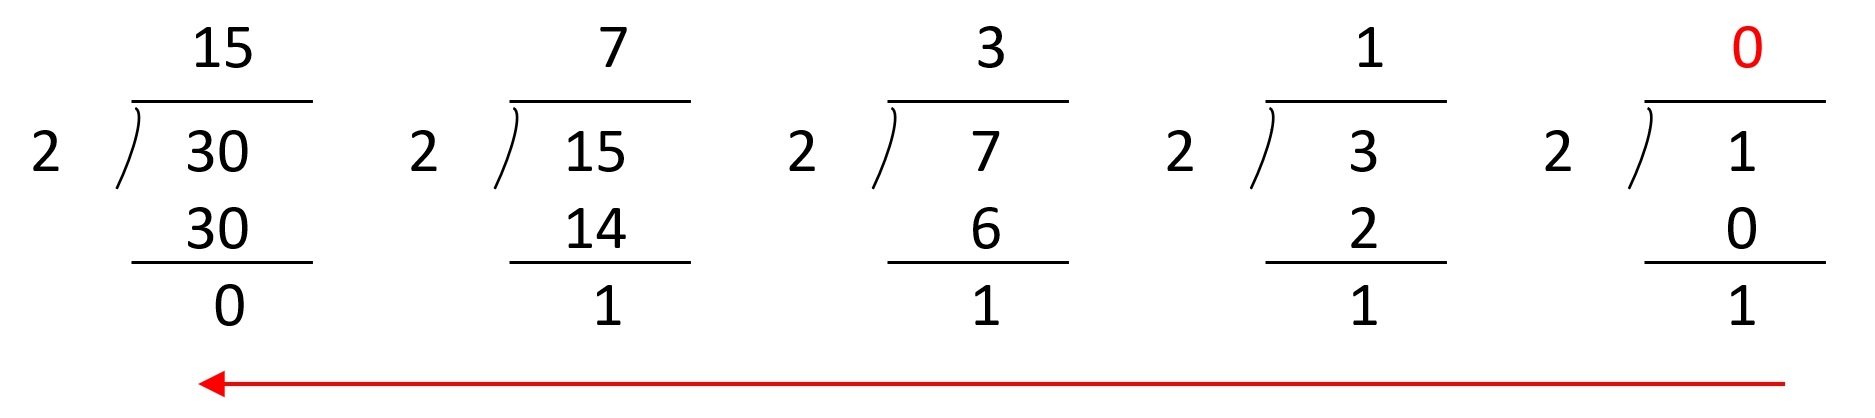
\includegraphics[width=.8\textwidth]{ch15/dec2bin.png}
    \end{itemize}

\end{frame}
%------------------------------------------------------------

%------------------------------------------------------------
\begin{frame}[fragile]
    \frametitle{十进制转二进制}

    \begin{itemize}
        \item $(10011)_{2} = 1 \times 2^4 + 0 \times 2^3 + 0 \times 2^2 + 1 \times 2^1 + 1 \times 2^0$
    \end{itemize}
    
    \only<1-2>{
        \centering
        \renewcommand{\arraystretch}{1.2} %设置垂直内边距为1.2倍默认行高
        \begin{tabular}{|c|c|c|c|c|c|}
        \hline
        数位  & 1 & 0 & 0 & 1 & \textcolor{red}{1} \\ \hline
        权重  & $2^4$ & $2^3$ & $2^2$ & $2^1$ & \textcolor{red}{$2^0$(值为 $1$)}  \\ \hline
        加数 & $1 \times 2^4$ & $0 \times 2^3$ & $0 \times 2^2$ & $1 \times 2^1$ & \textcolor{red}{$1 \times 2^0$}  \\ \hline
        \end{tabular}
    }  
    \only<3-4>{
        \centering
        \renewcommand{\arraystretch}{1.2} %设置垂直内边距为1.2倍默认行高
        \begin{tabular}{|c|c|c|c|c|}
        \hline
        数位  & 1 & 0 & 0  & \textcolor{red}{1} \\ \hline
        权重  & $2^3$ & $2^2$ & $2^1$ & \textcolor{red}{$2^0$(值为 $1$)}  \\ \hline
        加数  & $1 \times 2^3$ & $0 \times 2^2$ & $0 \times 2^1$ & \textcolor{red}{$1 \times 2^0$}  \\ \hline
        \end{tabular}
    }  
    \only<5>{
        \centering
        \renewcommand{\arraystretch}{1.2} %设置垂直内边距为1.2倍默认行高
        \begin{tabular}{|c|c|c|c|}
        \hline
        数位  & 1 & 0  & \textcolor{red}{0} \\ \hline
        权重  & $2^2$ & $2^1$ & \textcolor{red}{$2^0$(值为 $1$)}  \\ \hline
        加数  & $1 \times 2^2$ & $0 \times 2^1$ & \textcolor{red}{$0 \times 2^0$}  \\ \hline
        \end{tabular}
    }  
    \only<6>{
        \centering
        \renewcommand{\arraystretch}{1.2} %设置垂直内边距为1.2倍默认行高
        \begin{tabular}{|c|c|c|}
        \hline
        数位  & 1   & \textcolor{red}{0} \\ \hline
        权重  & $2^1$ & \textcolor{red}{$2^0$(值为 $1$)}  \\ \hline
        加数  & $1 \times 2^1$ & \textcolor{red}{$0 \times 2^0$}  \\ \hline
        \end{tabular}
    }  
    \only<7>{
        \centering
        \renewcommand{\arraystretch}{1.2} %设置垂直内边距为1.2倍默认行高
        \begin{tabular}{|c|c|}
        \hline
        数位  & \textcolor{red}{1} \\ \hline
        权重  & \textcolor{red}{$2^0$(值为 $1$)}  \\ \hline
        加数  & \textcolor{red}{$1 \times 2^0$}  \\ \hline
        \end{tabular}
    }  
    
    \begin{itemize}
        \item<2-> $\% 2$ 得到二进制数的最低位
        \item<3-> $/ 2$ 去掉二进制数的最低位
        \item<4-> 重复以上步骤 不断得到二进制的每一位
    \end{itemize}

\end{frame}
%------------------------------------------------------------

%------------------------------------------------------------
\begin{frame}[fragile]
    \frametitle{除二取余法}

    \begin{itemize}
        \item 联系十进制数位拆分的写法
        \begin{itemize}
           \item 对一个数值 $n$ 在循环中重复 \lstinline|n % 10, n /= 10| 的操作,可以得到这个数值十进制逆序的每一位
           \item 对一个数值 $n$ 在循环中重复 \lstinline|n % 2, n /= 2| 的操作,可以得到这个数值二进制逆序的每一位
        \end{itemize}
        
        \item \textbf{口诀:模二除二,逆序输出}
    \end{itemize}

\end{frame}
%------------------------------------------------------------

%------------------------------------------------------------
\begin{frame}[fragile]
    \frametitle{例 3.2:十进制转二进制}

    \alt<2-4>{
         \alt<2-3>{
            \lstinputlisting[basicstyle=\ttfamily\scriptsize,language=C++,name=dec2bin]{ch15/dec2bin.cc}
            
            \begin{tikzpicture}[remember picture,overlay]
                \uncover<3>{\redbox{dec2bin}{8}{5}{9}{21};}
                \uncover<3>{\redbox{dec2bin}{13}{8}{13}{31};}
            \end{tikzpicture}
        }{
            \lstinputlisting[basicstyle=\ttfamily\scriptsize,language=C++,name=dec2bin_2]{ch15/dec2bin_2.cc}
        }
    }{
        \begin{exampleblock}{编程题}

            \begin{itemize}
                \item 输入一个十进制表示的非负整数 $n$ ($0 \le n \le 10^9$),输出其二进制数值。

                \item 样例输入

                    \lstinline|30|

                \item 样例输出

                    \lstinline|11110|

            \end{itemize}

        \end{exampleblock}
    }
\end{frame}
%------------------------------------------------------------

%------------------------------------------------------------
\begin{frame}[fragile]
    \frametitle{二进制与十进制的转换}

    \begin{itemize}
        \item 二进制整数转十进制整数
        
            \begin{itemize}
                \item 按权展开求和
            \end{itemize}

        \item 十进制整数转二进制整数
        
            \begin{itemize}
                \item 模二除二,逆序输出
            \end{itemize}
    \end{itemize}
\end{frame}
%------------------------------------------------------------

\section{其他进制整数与十进制整数的转换}

%------------------------------------------------------------
\begin{frame}[fragile]
    \frametitle{八进制转十进制}

    \begin{itemize}
        \item  $(107)_{8}$ 按权展开是怎样的?
        \begin{itemize}
           \item \alt<1>{$1 \times 2^2 + 0 \times 2^1 + 7 \times 2^0$}{\redout{$1 \times 2^2 + 0 \times 2^1 + 7 \times 2^0$}}
           \item \alt<1>{$1 \times 8^0 + 0 \times 8^1 + 7 \times 8^2$}{\redout{$1 \times 8^0 + 0 \times 8^1 + 7 \times 8^2$}}
           \item $1 \times 8^2 + 0 \times 8^1 + 7 \times 8^0$
        \end{itemize}
        \item<3-> 八进制各个数位的权重是 $8$ 的幂,高位权重大于低位权重
        \item<4-> 八进制转十进制的方法同样是按权展开求和
        \begin{itemize}
           \item 列出展开式,计算其的十进制数值
        \end{itemize}
    \end{itemize}

\end{frame}
%------------------------------------------------------------

%------------------------------------------------------------
\begin{frame}[fragile]
    \frametitle{十六进制转十进制}

    \begin{itemize}[<+->]
        \item  $X$ 进制转十进制的方法都是按权展开求和
        \item 十六进制各个数位的权重是 $16$ 的幂
        \item 十六进制通常用 $A \sim F$ 或 $a \sim f$ 表示 $10 \sim 15$ ,展开时要将字母转换成对应的数字
        \item $(A2)_{16} = ?$
        \begin{itemize}
           \item $(A2)_{16} = 10 \times 16^1 + 2 \times 16^0 = 162$
        \end{itemize}
    \end{itemize}

\end{frame}
%------------------------------------------------------------

%------------------------------------------------------------
\begin{frame}[fragile]
    \frametitle{十进制转八进制}

    \begin{itemize}
        \item 十进制转二进制用“除二取余法”,十进制转八进制应该用什么方法?
        \item 除八取余法
        \item $(207)_{10} = ?$
        \begin{itemize}
           \item $207 \div 8 = 25 \dots 7$
           \item $25 \div 8 = 3 \dots 1$
           \item $3 \div 8 = 0 \dots 3$
           \item 余数逆序,可得其八进制 $(317)_8$
        \end{itemize}
    \end{itemize}

\end{frame}
%------------------------------------------------------------

%------------------------------------------------------------
\begin{frame}[fragile]
    \frametitle{十进制转十六进制}

    \begin{itemize}
        \item 十进制转 $X$ 进制的方法都是除 $X$ 取余法
        \item 算出来的余数是大于等于 $10$ 的数字要转换成对应的字母
        \item $(719)_{10} = ?$
        \begin{itemize}
           \item $719 \div 16 = 44 \dots 15(F)$
           \item $44 \div 16 = 2 \dots 12(C)$
           \item $2 \div 16 = 0 \dots 2$
           \item 余数逆序,可得其八进制 $(2CF)_{16}$
        \end{itemize}
    \end{itemize}

\end{frame}
%------------------------------------------------------------

\section{实数的进制转换}

%------------------------------------------------------------
\begin{frame}[fragile]
    \frametitle{二进制实数转十进制}

    \begin{itemize}[<+->]
        \item $(10.101)_2$ 按权展开是怎样的?
        \begin{align*}
        (10.101)_2 &= 1 \times 2^1 + 0 \times 2^0 + 1 \times 2^{-1} + 0 \times 2^{-2} + 1 \times 2^{-3} \\
                   &= 1 \times 2 + 0 \times 1 + 1 \times 0.5 + 0 \times 0.25 + 1 \times 0.125 \\
                   &= (2.625)_{10}
        \end{align*}
    \end{itemize}

\end{frame}
%------------------------------------------------------------

%------------------------------------------------------------
\begin{frame}[fragile]
    \frametitle{十进制实数转二进制}

    \begin{itemize}[<+->]
        \item 整数部分用\textbf{除二取余法},小数部分用\textbf{乘二取整法}
        \item 以 $(2.375)_{10}$ 为例
        \begin{itemize}
            \item 整数部分 $(2)_2$ 转十进制为 $(10)_2$
            \item 小数部分 $(0.375)_{10}$ 使用乘二取整法:
            \begin{itemize}
                \item $0.375 \times 2 = 0.75$
                \item $0.75 \times 2 = 1.5$
                \item $0.5 \times 2 = 1.0$
                \item 直到小数部分为 $.0$ 时停止计算
                \item 小数部分转二进制的结果:顺序记下商的整数部分 $(0.011)_2$
            \end{itemize}
            \item $(2.375)_{10} = (10.011)_2$
        \end{itemize}
    \end{itemize}

\end{frame}
%------------------------------------------------------------

%------------------------------------------------------------
\begin{frame}[fragile]
    \frametitle{实数储存的精度问题}

    \begin{itemize}[<+->]
        \item 计算机储存数字都是以二进制形式储存
        \item 以 $(0.6)_{10}$ 转换为二进制为例
        \begin{itemize}
            \item $0.6 \times 2 = 1.2$
            \item $0.2 \times 2 = 0.4$
            \item $0.4 \times 2 = 0.8$
            \item $0.8 \times 2 = 1.6$
            \item 计算过程进入无限循环,无法用有限位二进制准确表示
        \end{itemize}
    \end{itemize}

\end{frame}
%------------------------------------------------------------

%------------------------------------------------------------
\begin{frame}[fragile]
    \frametitle{实数储存的精度问题}

    \begin{itemize}[<+->]
        \item \lstinline|double| 类型只保证 $15$ 位有效数字的精度
        \item 平时尽量避免浮点数计算
        \begin{itemize}
            \item 可用 $i * i <= n$ 替代 $i <= sqrt(n)$
        \end{itemize}
        \item 若需判断浮点数是否相等,需要允许微小误差
        \begin{itemize}
            \item 需用 \lstinline|if (abs(a - b) < 1e-10)| 替代 \lstinline|if (a == b)|
        \end{itemize}
    \end{itemize}

\end{frame}
%------------------------------------------------------------

\section{总结}

%------------------------------------------------------------
\begin{frame}[fragile]
    \frametitle{进制}

    \begin{itemize}
        \item<1-> 进制
        
            \begin{itemize}
                \item 基数、数码、权重、数值、二进制的加减乘除
            \end{itemize}

        \item<2-> 进制转换
        
            \begin{itemize}
                \item 二进制整数转十进制(按权展开求和)
                \item 十进制整数转二进制(除二取余法)
                \item $X$ 进制整数转十进制(按权展开求和)
                \item 十进制整数转 $X$ 进制(除 $X$ 取余法)
            \end{itemize}
       
        \item<3-> 实数储存有精度问题,应避免进行浮点数运算
    \end{itemize}
\end{frame}
%------------------------------------------------------------

%------------------------------------------------------------
\begin{frame}
    \begin{center}
        {\Huge Thank you!}
    \end{center}
\end{frame}
%------------------------------------------------------------

\end{document}
